\section{D. Irga B. Naufal Fakhri}
\subsection{Pemahaman Teori}
\begin{enumerate}
\item Apa itu fungsi library matplotlib

	Matplotlib adalah modul python untuk menggambar plot 2D dengan kualitas tinggi. matplotlib dapat digunakan dalam script python, interpreter python dan ipython, server, dan 6 GUI toolkit. matplotlib berusaha untuk membuat segalanya jadi mudah, dan yang tadinya seperti tidak menjadi mungkin untuk dilakukan. Dengan matplotlib, Anda dapat membuat plots, histograms, spectra, bar charts, errorchards, scatterplots, dan masih banyak lagi.

\item Jelaskan langkah-langkah membuat sumbu X dan Y di matplotlib
\begin{enumerate}
	\item pertama import dulu library matplotlib lalu beri alias plt
	\lstinputlisting[firstline=7, lastline=7]{src/6/1174066/Teori/1174066.py}
	
	\item Kemudian buat variable array x dengan isi terserah anda
	\lstinputlisting[firstline=8, lastline=8]{src/6/1174066/Teori/1174066.py}
	
	\item Lalu buat variable array y juga dengan isi terserah anda yang penting jumlahnya sama dengan variable X
	\lstinputlisting[firstline=9, lastline=9]{src/6/1174066/Teori/1174066.py}
	
	\item Kemudian buat plot berisikan variable x dan y pada modul plt
	\lstinputlisting[firstline=10, lastline=10]{src/6/1174066/Teori/1174066.py}
	
	\item Yang terakhir, munculkan plot yang telah kita buat dengan fungsi show()
	\lstinputlisting[firstline=11, lastline=11]{src/6/1174066/Teori/1174066.py}
\end{enumerate}

\item Jelaskan bagaimana perbedaan fungsi dan cara pakai untuk berbagai jenis(bar,histogram,scatter,line dll) jenis plot di matplotlib

	Perbedaan pada fungsi plot adalah pada bentuk gambar grafik yang dihasilkan pada program dan jenis jenis grafik yang ada pada plot adalah:
\begin{itemize}
	\item Plot
		
	Grafik yang dihasilkan oleh plot ini adalah sebuah garis (line)
	\lstinputlisting[firstline=7, lastline=11]{src/6/1174066/Teori/1174066.py}
	
	\item Bar
	
	Grafik yang dihasilkan oleh bar adalah sebuah bentuk grafik batang (bar) dan cara penggunaan bar adalah menggunakan fungsi bar(variable x, variable y)
	\lstinputlisting[firstline=14, lastline=18]{src/6/1174066/Teori/1174066.py}
	
	\item Histogram
	
	Dalam penggunaaan histogram yaitu menggunakan .hist(variable x, variable y) dengan variable x berisikan data dan variable y berisikan keliapatan yang akan dimunculkan pada histogram
	\lstinputlisting[firstline=21, lastline=24]{src/6/1174066/Teori/1174066.py}
	
	\item Scatter
	
	Grafik yang dihasilkan oleh scatter adalah diagram titik dan cara penggunaannya menggunakan .scatter(variable x, variable y)
	\lstinputlisting[firstline=27, lastline=39]{src/6/1174066/Teori/1174066.py}
	
	\item Stack Plot
	
	Grafik yang dihasilkan oleh stack plot ini hampir sama seperti diagram line, hanya hasil datanya disatuin semua keatasnya dan cara penggunaannya adalah menggunakan .stackplot(variable, variable, variable)
	\lstinputlisting[firstline=41, lastline=58]{src/6/1174066/Teori/1174066.py}
\end{itemize}

\item Jelaskan bagaimana cara menggunakan legend dan label serta kaitannya dengan fungsi tersebut

	Cara menggunakan legend adalah namaObject.legend() dan menambahkan labelnya seperti dibawah ini:
\lstinputlisting[firstline=54, lastline=58]{src/6/1174066/Teori/1174066.py}
Penggunaan legend itu berfungsi untuk memudahkan kita ketika membaca grafik yang kita hasilkan karena kita memberi nama pada data yang ditampilkan sama seperti label kita memberikan nama kepada variable yang dimunculkan di grafik dan membedakan antara variable yang satu dengan yang lain, kita juga bisa menambahkan warna ke label

\item Jelaskan apa fungsi dari subplot di matplotlib, dan bagaimana cara kerja dari fungsi subplot, sertakan ilustrasi dan gambar sendiri dan apa parameternya jika ingin menggambar plot dengan 9 subplot di dalamnya

	Subplot berfungsi untuk menampikan grafik plot pada program yang sama, cara penggunaannya:
\lstinputlisting[firstline=60, lastline=70]{src/6/1174066/Teori/1174066.py}
Cara penggunaannya sebagai contoh saya ambil plt.subplot(221), pada angka 2 yang pertama adalah pembagian keatas kalo kita mau bagi 3 keatas kita isi angka pertama dengan 3, angka 2 yang kedua adalah pembagian kesamping penggunaannya sama kaya angka pertama kalo kita mau ngebagi kesamping 4 kita isi angka kedua 4, dan angka 1 pada angka ketiga itu tempat disimpannya grafik yang akan dimunculkan

\item Sebutkan semua parameter color yang bisa digunakan (contoh: m,c,r,k,... dkk)

	Parameter warna yang bisa digunakan dibagi menjadi 2 tipe:
\begin{itemize}
	\item RGB
	
	Untuk keterangannya sebagai berikut
    R untuk warna Red atau Merah
    G untuk warna Green atau Hijau
    B untuk warna Blue atau Biru
    
    \item CMYK
    
    Untuk keterangannya sebagai berikut
    C untuk warna Cyan atau Biru Muda
    M untuk warna Mangenta atau Merah Tua
    Y untuk warna Yellow Atau Kuning
    K untuk warna Black atau Hitam
\end{itemize}

\item Jelaskan bagaimana cara kerja dari fungsi hist, sertakan ilustrasi dan gambar sendiri

	Untuk histogram kita tidak boleh memiliki is variable x dan y yang sama. Misal x-nya ada 10 nilai sedangkan Y-nya ada 5 nilai, data tersebut tidak menjadi masalah karena pada histogram data yang dimunculkan adalah data rentang dari data variable y. Dan ini adalah contoh dari penggunaan histogram
\lstinputlisting[firstline=82, lastline=87]{src/6/1174066/Teori/1174066.py}

\item Jelaskan lebih mendalam tentang parameter dari fungsi pie diantaranya labels, colors, startangle, shadow, explode, autopct

\begin{itemize}
    \item Label
    
    Label digunakan untuk mempermudah pembaca yaitu memberikan nama pada variable di grafik
    
    \item Color
    
    Warna yang dimunculkan pada setiap data
    
    \item Startangle
    
    Startangle digunakan untuk sudut awal pada diagram pie tersebut
    
    \item Shadow
    
    Shadow(Bayangan) digunakan untuk membuat bayangan pada setiap diagram pie yang menonjol
    
    \item Explode

    Explode digunakan untuk mengeluarkan suatu data agar data tersebut menjadi terlihat lebih menonjol
    
    \item Autopct
    
    Autopct digunakan menyesuaikan berapa angka yang ada dibelakang koma
\end{itemize}
\end{enumerate}

%%%%%%%%%%%%%%%%%%%%%%%%%%%%%%%%%%%%%%%%%%%%%%%%%%%%%%%%%%%%%%%%%%%%%%%%%%%%%%%%%%%%%%%%%%%%%%%%%%%%%%%%%%%%%%%%%%%%%%%%%%

\section{Fanny Shafira Damayanti | 1174069}
\subsection{Pemahaman Teori}
\begin{enumerate}
\item Fungsi Library matplotlib

matplotlib adalah librari plotting 2D Python yang menghasilkan gambar publikasi bermutu di dalam berbagai format hardcopy dan lingkungan interaktif sepanjang platform. matplotlib dapat digunakan di dalam script Python, shell Python dan ipython.

\item Langkah - langkah membuat sumbu X dan Y di matplotlib

caranya yaitu seperti contoh dibawah ini :
\lstinputlisting[firstline=9, lastline=10]{src/6/1174069/Teori/1174069_teori.py}

\item Perbedaan fungsi dan cara pakai untuk berbagai jenis (bar, histogram, scatter,dll) jenis plot di matplotlib

Perbedaannya adalah bentuk bentuk grafik yang akan di tampilkan sesuai dengan perintah yang digunakan pada pemogramannya.

cara pengguna plot tersebut sebagai berikut :

\begin{itemize}
    \item line
    Perintah yang digunakan untuk membuat grafik line sebagai berikut.
    \lstinputlisting[firstline=12, lastline=14]{src/6/1174069/Teori/1174069_teori.py}
	
    \item bar
    Memiliki koordinat X dan Koordinat Y
	\lstinputlisting[firstline=16, lastline=25]{src/6/1174069/Teori/1174069_teori.py}
    
    \item histogram
    Dalam penggunaan plot histogram titik x nya bisa tidak sama dengan titik Y.
    \lstinputlisting[firstline=27, lastline=34]{src/6/1174069/Teori/1174069_teori.py}
   
    \item scatter
   Penggunaan plot scatter atau bisa juga di bilang diagram titik.
   \lstinputlisting[firstline=36, lastline=49]{src/6/1174069/Teori/1174069_teori.py}
    
    \item Stack plot
    Untuk penggunaan stack plot ini seperti diagram line, tapi ada fill colornya,jadi antar line itu bisa berdekatan.
	\lstinputlisting[firstline=82, lastline=92]{src/6/1174069/Teori/1174069_teori.py}
    
\end{itemize}

\item Cara menggunakan legend dan label serta kaitannya dengan fungsi tersebut

Legend digunakan untuk mempermudah dalam membaca grafik, legend itu sendiri berisi info info dari grafik yang ada seperti nama, kemudian bentuk dan warna.
kemudian untuk label itu sendiri digunakan untuk membedakan nama titik X dan titik Y.

Contohnya sebagai berikut :
\lstinputlisting[firstline=20, lastline=22]{src/6/1174069/Teori/1174069_teori.py}

\item Fungsi dari subplot di matplotlib, dan cara kerja dari fungsi subplot sertakan contoh gambarnya

fungsi subplot di matplotlib yaitu untuk bisa membuat lebih dari 1 grafik dalam sebuah program.
Contohnya :
\lstinputlisting[firstline=94, lastline=104]{src/6/1174069/Teori/1174069_teori.py}

\begin{figure}[H]	
    \includegraphics[width=5cm]{figures/6/1174069/Teori/chart.png}
    \centering
    \caption{SubPlot}
\end{figure}

\item Paramater color yang bisa digunakan

\begin{itemize}
    \item Tipe Warna RGB

    R untuk warna Red atau Merah
    G untuk warna Green atau Hijau
    B untuk warna Blue atau Biru
    \item Tipe warna CMYK

    C untuk warna Cyan atau Biru Muda
    M untuk warna Mangenta atau Merah Tua
    Y untuk warna Yellow Atau Kuning
    K untuk warna black atau Hitam
\end{itemize}

\item Cara kerja dari fungsi hist, sertakan ilustrasi dan gambar sendiri

Untuk fungsi histogram ini kedua titik koordinat boleh tidak sama. Misalnya x nya ada 10 nilai sedangkan Y nya ada 5 nilai, itu tidak akan jadi masalah karena diagram ini digunakan untuk mendata usia dari rentang tertentu atau kebutuhan lainnya.
Contoh penggunaan histogram :
\lstinputlisting[firstline=27, lastline=34]{src/6/1174069/Teori/1174069_teori.py}

Contoh grafiknya :
\begin{figure}[H]	
    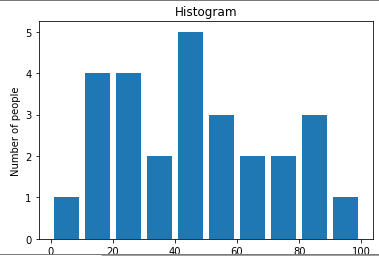
\includegraphics[width=5cm]{figures/6/1174069/Teori/histogram.png}
    \centering
    \caption{Diagram Histogram}
\end{figure}

\item Parameter dari fungsi pie diantaranya labels, colors, startangle, shadow, explode, autopct

\begin{itemize}
    \item label
    Label digunakan untuk mempermudah pembaca dalam membaca diagram pie
    \item color
    warna digunakan untuk membedakan antar data
    \item startangle
    Digunakan untuk sudut yang digunakan untuk memulai diagram pie tersebut
    \item shadow
    bayangan digunakan untuk membuat bayangan dari setiap diagram pie yang menonjol
    \item explode
    explode digunakan untuk mengeluarkan suatu data agar data tersebut terlihat menonjol
    \item autopct
    Digunakan sesuai dengan berapa angka dibelakang koma yang kita inginkan
\end{itemize}

\end{enumerate}

